\documentclass[12pt,a4paper]{article}
\usepackage[margin=2cm]{geometry}
\usepackage{enumitem}
\usepackage{xcolor}
\usepackage{booktabs}
\usepackage{tikz}
\usetikzlibrary{arrows.meta, positioning, shapes.geometric}
\usepackage{hyperref}
\hypersetup{colorlinks=true, linkcolor=blue, urlcolor=blue}

\definecolor{phase1}{RGB}{220,240,255}
\definecolor{phase2}{RGB}{255,240,220}
\definecolor{phase3}{RGB}{220,255,220}
\definecolor{phase4}{RGB}{255,220,220}
\definecolor{phase5}{RGB}{240,220,255}
\definecolor{lc1}{RGB}{200,230,255}
\definecolor{lc2}{RGB}{255,230,200}
\definecolor{lc3}{RGB}{200,255,200}

\title{Project Flowcycle: Complete Reading, Preparation \& Presentation Schedule\\[0.3cm]
\large From Zero Knowledge to Showing Output --- With Dates}
\author{Landslide Identification Using ML}
\date{}

\begin{document}
\maketitle

\section*{How to Use This File}

This is your \textbf{master roadmap with a day-by-day schedule}. It tells you exactly what to read, in what order, and \textbf{when to do each task} so you are fully prepared for all three lifecycle presentations.

\vspace{0.3cm}
\noindent\fcolorbox{black}{red!10}{%
\parbox{\dimexpr\linewidth-2\fboxsep-2\fboxrule}{%
\textbf{Your Deadlines:}\\[0.2cm]
\begin{tabular}{lll}
    \textbf{Lifecycle 1} & Saturday, 21 March 2026 & (3 days from today) \\
    \textbf{Lifecycle 2} & Saturday, 29 March 2026 & (suggested) \\
    \textbf{Lifecycle 3} & Sunday, 7 April 2026 & (final deadline --- 20 days total) \\
\end{tabular}
}}

\vspace{0.3cm}
\noindent\fcolorbox{black}{yellow!15}{%
\parbox{\dimexpr\linewidth-2\fboxsep-2\fboxrule}{%
\textbf{Quick Path:} Files marked with $\bigstar$ are must-reads. If short on time for any lifecycle, read only $\bigstar$ files.
}}

% ============================================================
% ============================================================
\part*{LIFECYCLE 1 PREPARATION}
\addcontentsline{toc}{part}{Lifecycle 1 Preparation}
% ============================================================
% ============================================================

\noindent\fcolorbox{black}{lc1}{%
\parbox{\dimexpr\linewidth-2\fboxsep-2\fboxrule}{%
\centering\Large\textbf{LIFECYCLE 1 --- Present on Saturday, 21 March 2026}\\[0.1cm]
\normalsize Foundation \& Baseline Models (r0, r1, r2)\\
\textbf{Covers:} Problem statement, pipeline design, AlexNet, EfficientNet-B3
}}

% ---- Day 1 ----
\section{Day 1: Wednesday, 19 March 2026 --- Learn the Basics}

\noindent\textit{Goal: Understand WHY this project exists and learn all ML terms you need.}

\begin{center}
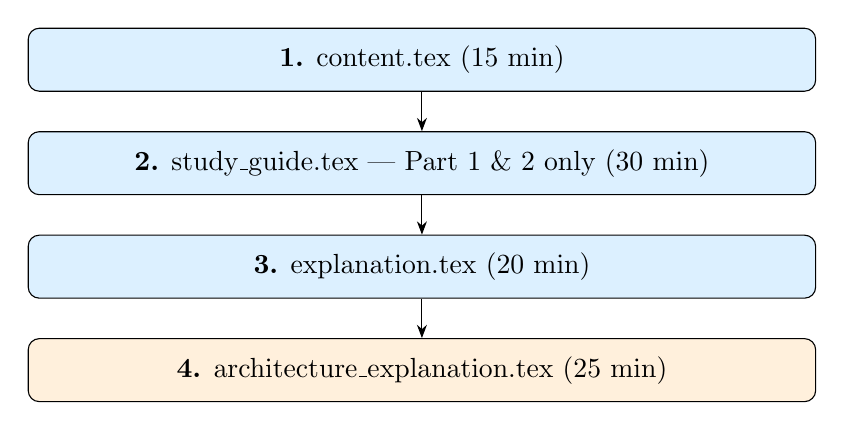
\begin{tikzpicture}[
    node distance=0.5cm,
    box/.style={rectangle, draw, rounded corners, minimum width=10cm, minimum height=0.8cm, align=center, fill=#1}
]
\node[box=phase1] (a) {\textbf{1.} content.tex (15 min)};
\node[box=phase1, below=of a] (b) {\textbf{2.} study\_guide.tex --- Part 1 \& 2 only (30 min)};
\node[box=phase1, below=of b] (c) {\textbf{3.} explanation.tex (20 min)};
\node[box=phase2, below=of c] (d) {\textbf{4.} architecture\_explanation.tex (25 min)};
\draw[-{Stealth}] (a) -- (b);
\draw[-{Stealth}] (b) -- (c);
\draw[-{Stealth}] (c) -- (d);
\end{tikzpicture}
\end{center}

\subsection*{Step 1: content.tex $\bigstar$}
\begin{itemize}[leftmargin=1.5cm]
    \item[\textbf{Time:}] 15 minutes
    \item[\textbf{What you learn:}] Why landslide detection matters. Real-world impact (thousands killed, millions displaced). Why existing methods (manual interpretation, NDVI, SVM) are not enough. What gap this project fills.
    \item[\textbf{After reading, you can answer:}]
    \begin{itemize}
        \item Why did you choose this project?
        \item What is the real-world problem?
        \item How is your approach different from existing methods?
    \end{itemize}
\end{itemize}

\subsection*{Step 2: study\_guide.tex (Part 1 \& 2 only) $\bigstar$}
\begin{itemize}[leftmargin=1.5cm]
    \item[\textbf{Time:}] 30 minutes
    \item[\textbf{What you learn:}] What is ML, neural networks, CNN, transfer learning, HMM. All terms in simple English. Key metrics table (accuracy, precision, recall, F1, AUC).
    \item[\textbf{After reading, you can answer:}]
    \begin{itemize}
        \item What is a CNN? What is a convolution?
        \item What is transfer learning and why is it useful?
        \item What does each metric measure?
        \item What is an HMM and why use it here?
    \end{itemize}
\end{itemize}

\subsection*{Step 3: explanation.tex}
\begin{itemize}[leftmargin=1.5cm]
    \item[\textbf{Time:}] 20 minutes
    \item[\textbf{What you learn:}] The two-phase pipeline explained simply --- Phase 1 (image in, landslide/non-landslide out) and Phase 2 (country data in, risk forecast out). How they connect.
\end{itemize}

\subsection*{Step 4: architecture\_explanation.tex $\bigstar$}
\begin{itemize}[leftmargin=1.5cm]
    \item[\textbf{Time:}] 25 minutes
    \item[\textbf{What you learn:}] Technical details --- CNN layers, pooling, FC layers. AlexNet vs EfficientNet-B3 differences. HMM hidden states and observations. Flow diagrams.
    \item[\textbf{After reading, you can answer:}]
    \begin{itemize}
        \item How does your CNN classify images?
        \item What is EfficientNet-B3? How is it different from AlexNet?
        \item How does the HMM work?
    \end{itemize}
\end{itemize}

\vspace{0.3cm}
\noindent\textbf{Day 1 Checkpoint:} You understand the problem, know all ML terms, and can explain the pipeline and architecture. \textbf{Total: $\sim$1.5 hours.}

% ---- Day 2 ----
\section{Day 2: Thursday, 20 March 2026 --- Learn LC1 Results + Q\&A Prep}

\noindent\textit{Goal: Understand the three LC1 experiments and prepare for questions.}

\begin{center}
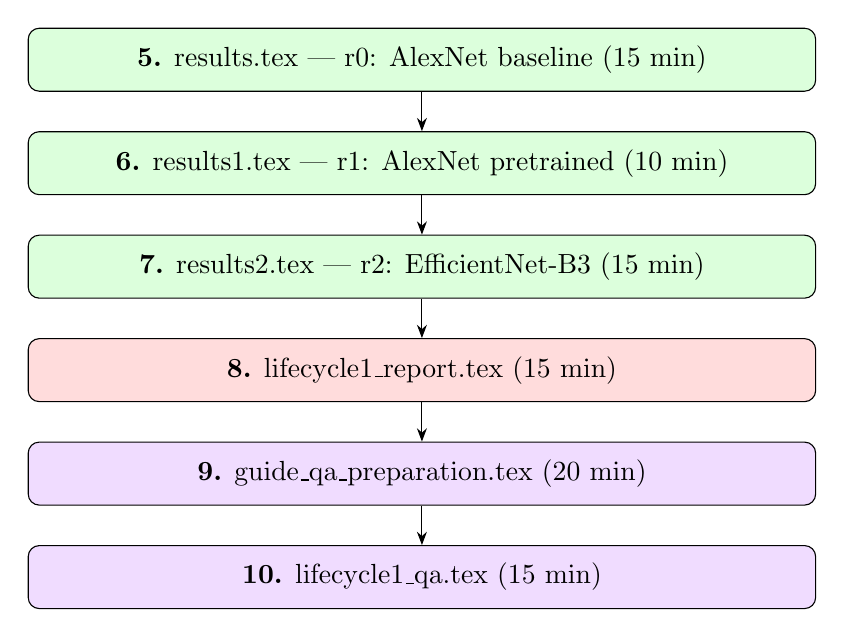
\begin{tikzpicture}[
    node distance=0.5cm,
    box/.style={rectangle, draw, rounded corners, minimum width=10cm, minimum height=0.8cm, align=center, fill=#1}
]
\node[box=phase3] (a) {\textbf{5.} results.tex --- r0: AlexNet baseline (15 min)};
\node[box=phase3, below=of a] (b) {\textbf{6.} results1.tex --- r1: AlexNet pretrained (10 min)};
\node[box=phase3, below=of b] (c) {\textbf{7.} results2.tex --- r2: EfficientNet-B3 (15 min)};
\node[box=phase4, below=of c] (d) {\textbf{8.} lifecycle1\_report.tex (15 min)};
\node[box=phase5, below=of d] (e) {\textbf{9.} guide\_qa\_preparation.tex (20 min)};
\node[box=phase5, below=of e] (f) {\textbf{10.} lifecycle1\_qa.tex (15 min)};
\draw[-{Stealth}] (a) -- (b);
\draw[-{Stealth}] (b) -- (c);
\draw[-{Stealth}] (c) -- (d);
\draw[-{Stealth}] (d) -- (e);
\draw[-{Stealth}] (e) -- (f);
\end{tikzpicture}
\end{center}

\subsection*{Step 5: results.tex (r0) $\bigstar$}
\begin{itemize}[leftmargin=1.5cm]
    \item[\textbf{Time:}] 15 minutes
    \item[\textbf{What you learn:}] Baseline AlexNet from scratch. 78.54\% accuracy, 67.67\% F1. Why it is the starting point. Problems: overconfident, 54 missed landslides.
    \item[\textbf{Key numbers:}] Acc=78.54\%, Prec=62.06\%, Rec=74.41\%, F1=67.67\%, AUC=85.53\%
\end{itemize}

\subsection*{Step 6: results1.tex (r1)}
\begin{itemize}[leftmargin=1.5cm]
    \item[\textbf{Time:}] 10 minutes
    \item[\textbf{What you learn:}] Same AlexNet but with ImageNet pretrained weights. Transfer learning gives +1.57\% accuracy. But recall dropped --- pretrained model is more conservative.
    \item[\textbf{Key takeaway:}] Transfer learning helps but AlexNet is too old/simple.
\end{itemize}

\subsection*{Step 7: results2.tex (r2) $\bigstar$}
\begin{itemize}[leftmargin=1.5cm]
    \item[\textbf{Time:}] 15 minutes
    \item[\textbf{What you learn:}] EfficientNet-B3 with compound scaling. 300x300 input, 12M params (vs 62M). Recall 78.20\% (8 fewer missed landslides). AUC 88.93\%.
    \item[\textbf{Key takeaway:}] Modern architecture + transfer learning = big improvement. End of LC1.
\end{itemize}

\subsection*{Step 8: lifecycle1\_report.tex $\bigstar$}
\begin{itemize}[leftmargin=1.5cm]
    \item[\textbf{Time:}] 15 minutes
    \item[\textbf{What you learn:}] LC1 as a coherent story. What was the goal, what was done, results, gaps identified. This is the summary view.
\end{itemize}

\subsection*{Step 9: guide\_qa\_preparation.tex $\bigstar$}
\begin{itemize}[leftmargin=1.5cm]
    \item[\textbf{Time:}] 20 minutes
    \item[\textbf{What you learn:}] Common questions about deep learning fundamentals --- backpropagation, gradient descent, overfitting, batch normalization. Simple answers ready.
\end{itemize}

\subsection*{Step 10: lifecycle1\_qa.tex $\bigstar$}
\begin{itemize}[leftmargin=1.5cm]
    \item[\textbf{Time:}] 15 minutes
    \item[\textbf{What you learn:}] LC1-specific questions: ``Why AlexNet first?'', ``Why EfficientNet-B3?'', ``What is transfer learning?'', ``Explain your confusion matrix.'' Each has a ready answer.
\end{itemize}

\vspace{0.3cm}
\noindent\textbf{Day 2 Checkpoint:} You know all three LC1 experiments and can answer Q\&A. \textbf{Total: $\sim$1.5 hours.}

% ---- Day 3 ----
\section{Day 3: Friday, 20 March 2026 (Night) --- Presentation Prep + Live Demo}

\noindent\textit{Goal: Practice the presentation, test live demo, be ready for tomorrow.}

\begin{center}
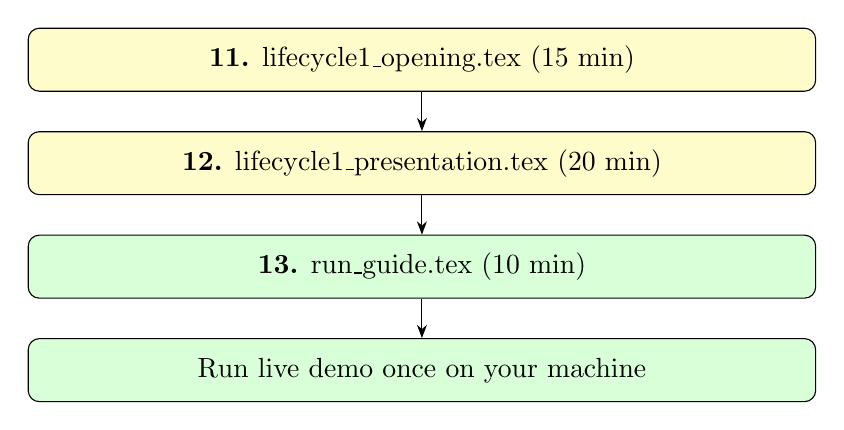
\begin{tikzpicture}[
    node distance=0.5cm,
    box/.style={rectangle, draw, rounded corners, minimum width=10cm, minimum height=0.8cm, align=center, fill=#1}
]
\node[box=yellow!20] (a) {\textbf{11.} lifecycle1\_opening.tex (15 min)};
\node[box=yellow!20, below=of a] (b) {\textbf{12.} lifecycle1\_presentation.tex (20 min)};
\node[box=green!15, below=of b] (c) {\textbf{13.} run\_guide.tex (10 min)};
\node[box=green!15, below=of c] (d) {Run live demo once on your machine};
\draw[-{Stealth}] (a) -- (b);
\draw[-{Stealth}] (b) -- (c);
\draw[-{Stealth}] (c) -- (d);
\end{tikzpicture}
\end{center}

\subsection*{Step 11: lifecycle1\_opening.tex $\bigstar$}
\begin{itemize}[leftmargin=1.5cm]
    \item[\textbf{Time:}] 15 minutes
    \item[\textbf{What you learn:}] How to START your presentation. Opening sentences, how to introduce the problem, speaking tips, confidence builders.
    \item[\textbf{Action:}] Read it out loud like a script. Practice 2--3 times.
\end{itemize}

\subsection*{Step 12: lifecycle1\_presentation.tex $\bigstar$}
\begin{itemize}[leftmargin=1.5cm]
    \item[\textbf{Time:}] 20 minutes
    \item[\textbf{What you learn:}] Your actual LC1 slides. 15 slides covering problem statement, pipeline, datasets, r0/r1/r2 results, output images, comparison table, key findings, LC2 preview.
    \item[\textbf{Action:}] Compile with \texttt{pdflatex lifecycle1\_presentation.tex} and click through every slide. Know what you will say on each.
\end{itemize}

\subsection*{Step 13: run\_guide.tex $\bigstar$}
\begin{itemize}[leftmargin=1.5cm]
    \item[\textbf{Time:}] 10 minutes
    \item[\textbf{Action:}] Read the commands, then actually run one prediction on your machine:
    \begin{enumerate}
        \item Open terminal in project folder
        \item Run: \texttt{python pipeline/run\_pipeline.py --mode predict --image data/processed/test/debris\_flow/ls\_test\_0011.jpg --country India --forecast 3}
        \item Verify you see Phase 1 detection + Phase 2 forecast output
        \item Open \texttt{project/plots/confusion\_matrix.png} and \texttt{roc\_curve.png}
    \end{enumerate}
\end{itemize}

\vspace{0.3cm}
\noindent\textbf{Day 3 Checkpoint:} Presentation practiced, live demo tested, you are ready.

% ---- Presentation Day ----
\section{PRESENTATION DAY: Saturday, 21 March 2026 --- Lifecycle 1}

\noindent\fcolorbox{black}{lc1}{%
\parbox{\dimexpr\linewidth-2\fboxsep-2\fboxrule}{%
\textbf{What to show your guide:}
\begin{enumerate}
    \item Open \textbf{lifecycle1\_presentation.tex} PDF --- present all slides
    \item Show \textbf{dataset samples} --- landslide vs non-landslide images
    \item Show \textbf{training\_history.png} --- training loss/accuracy curves
    \item Show \textbf{confusion\_matrix.png + roc\_curve.png} --- evaluation results
    \item Run \textbf{live prediction} on terminal --- show Phase 1 + Phase 2 output
    \item Show \textbf{comparison table} (r0 vs r1 vs r2) --- progression story
    \item End with: ``These are the gaps we found, and LC2 will address them''
\end{enumerate}
}}

\vspace{0.3cm}
\noindent\textbf{Last-minute revision (morning of 21 March):}
\begin{itemize}
    \item Re-read lifecycle1\_opening.tex --- practice opening 2 times
    \item Memorize: r0=78.54\%, r1=80.11\%, r2=79.97\% (but r2 has best recall and AUC)
    \item Memorize three sentences:
    \begin{itemize}
        \item ``We built a dual-phase pipeline: CNN detects landslides, HMM forecasts risk.''
        \item ``We improved from AlexNet to EfficientNet-B3, reducing missed landslides by 8.''
        \item ``The gaps we found --- overconfidence, single-model limits --- will be fixed in LC2.''
    \end{itemize}
    \item Run one prediction to confirm everything works
\end{itemize}

% ============================================================
% ============================================================
\part*{LIFECYCLE 2 PREPARATION}
\addcontentsline{toc}{part}{Lifecycle 2 Preparation}
% ============================================================
% ============================================================

\noindent\fcolorbox{black}{lc2}{%
\parbox{\dimexpr\linewidth-2\fboxsep-2\fboxrule}{%
\centering\Large\textbf{LIFECYCLE 2 --- Present on Saturday, 29 March 2026}\\[0.1cm]
\normalsize Optimization \& Ensemble Strategies (r3, r4, r5)\\
\textbf{Covers:} Temperature scaling, ensemble methods, ViT, optimal threshold
}}

\vspace{0.3cm}
\noindent You have \textbf{8 days} (22--29 March). Spread across 4 study sessions.

% ---- LC2 Day 1 ----
\section{Days 22--23 March (Mon--Tue) --- Learn LC2 Techniques}

\begin{center}
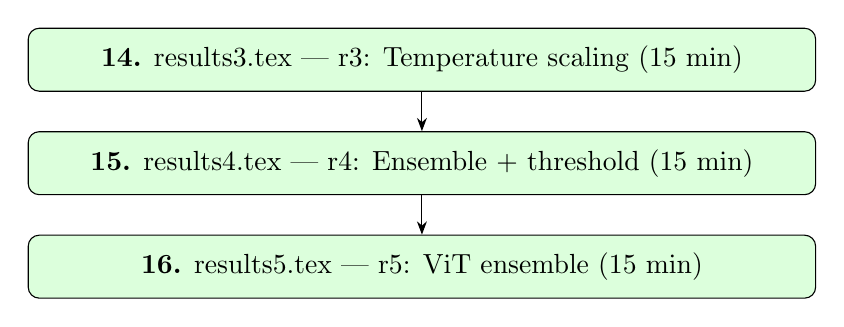
\begin{tikzpicture}[
    node distance=0.5cm,
    box/.style={rectangle, draw, rounded corners, minimum width=10cm, minimum height=0.8cm, align=center, fill=#1}
]
\node[box=phase3] (a) {\textbf{14.} results3.tex --- r3: Temperature scaling (15 min)};
\node[box=phase3, below=of a] (b) {\textbf{15.} results4.tex --- r4: Ensemble + threshold (15 min)};
\node[box=phase3, below=of b] (c) {\textbf{16.} results5.tex --- r5: ViT ensemble (15 min)};
\draw[-{Stealth}] (a) -- (b);
\draw[-{Stealth}] (b) -- (c);
\end{tikzpicture}
\end{center}

\subsection*{Step 14: results3.tex (r3) $\bigstar$}
\begin{itemize}[leftmargin=1.5cm]
    \item[\textbf{Time:}] 15 minutes
    \item[\textbf{What you learn:}] Temperature scaling: learned T=1.1511 on validation set. Divides logits by T before softmax. Does NOT change accuracy --- only fixes confidence. HMM upgraded to 8 states, 42 symbols.
    \item[\textbf{Key takeaway:}] 70\% confident now means actually 70\% accurate.
\end{itemize}

\subsection*{Step 15: results4.tex (r4) $\bigstar$}
\begin{itemize}[leftmargin=1.5cm]
    \item[\textbf{Time:}] 15 minutes
    \item[\textbf{What you learn:}] Ensemble: 60\% EfficientNet-B3 + 40\% AlexNet. Optimal threshold 46.7\% from PR curve. All 5 metrics improve.
    \item[\textbf{Key numbers:}] Acc=82.40\%, F1=72.97\%, AUC=89.83\%
\end{itemize}

\subsection*{Step 16: results5.tex (r5) $\bigstar$}
\begin{itemize}[leftmargin=1.5cm]
    \item[\textbf{Time:}] 15 minutes
    \item[\textbf{What you learn:}] Replace AlexNet with ViT-B/16. CNN sees local textures, ViT sees global patterns. Biggest single jump: F1 +3.01\%.
    \item[\textbf{Key numbers:}] Acc=84.55\%, F1=75.98\%, AUC=91.50\%
\end{itemize}

% ---- LC2 Day 2 ----
\section{Days 24--25 March (Wed--Thu) --- Reports + Deep Dives}

\begin{center}
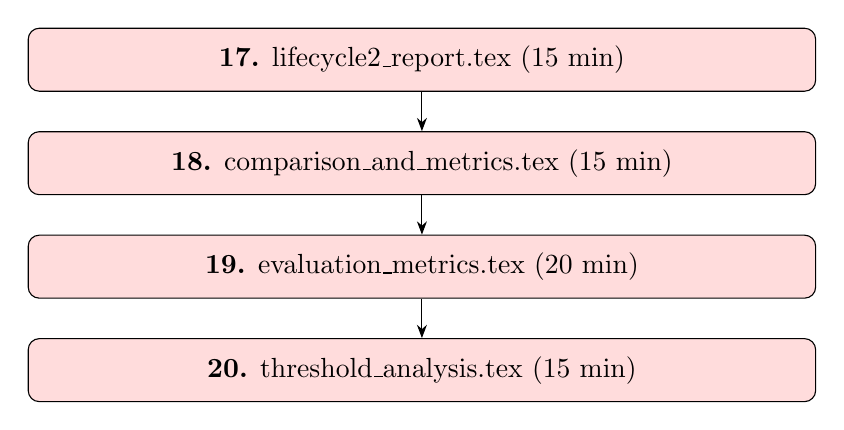
\begin{tikzpicture}[
    node distance=0.5cm,
    box/.style={rectangle, draw, rounded corners, minimum width=10cm, minimum height=0.8cm, align=center, fill=#1}
]
\node[box=phase4] (a) {\textbf{17.} lifecycle2\_report.tex (15 min)};
\node[box=phase4, below=of a] (b) {\textbf{18.} comparison\_and\_metrics.tex (15 min)};
\node[box=phase4, below=of b] (c) {\textbf{19.} evaluation\_metrics.tex (20 min)};
\node[box=phase4, below=of c] (d) {\textbf{20.} threshold\_analysis.tex (15 min)};
\draw[-{Stealth}] (a) -- (b);
\draw[-{Stealth}] (b) -- (c);
\draw[-{Stealth}] (c) -- (d);
\end{tikzpicture}
\end{center}

\subsection*{Step 17: lifecycle2\_report.tex $\bigstar$}
\begin{itemize}[leftmargin=1.5cm]
    \item[\textbf{Time:}] 15 minutes
    \item[\textbf{What you learn:}] LC2 as a complete story --- goals, methods, results, remaining gaps. Formal summary for your guide.
\end{itemize}

\subsection*{Step 18: comparison\_and\_metrics.tex}
\begin{itemize}[leftmargin=1.5cm]
    \item[\textbf{Time:}] 15 minutes
    \item[\textbf{What you learn:}] Side-by-side table of r0--r5. Exact metric deltas. Good for memorizing the progression.
\end{itemize}

\subsection*{Step 19: evaluation\_metrics.tex}
\begin{itemize}[leftmargin=1.5cm]
    \item[\textbf{Time:}] 20 minutes
    \item[\textbf{What you learn:}] Deep understanding of every metric with toy examples. Confusion matrix explained. ROC curve meaning. Why F1 is harmonic mean.
\end{itemize}

\subsection*{Step 20: threshold\_analysis.tex}
\begin{itemize}[leftmargin=1.5cm]
    \item[\textbf{Time:}] 15 minutes
    \item[\textbf{What you learn:}] Why 46.7\% and not 50\%. Precision-recall tradeoff. Good if guide asks about threshold.
\end{itemize}

% ---- LC2 Day 3 ----
\section{Days 26--27 March (Fri--Sat) --- Q\&A Prep + Presentation Practice}

\begin{center}
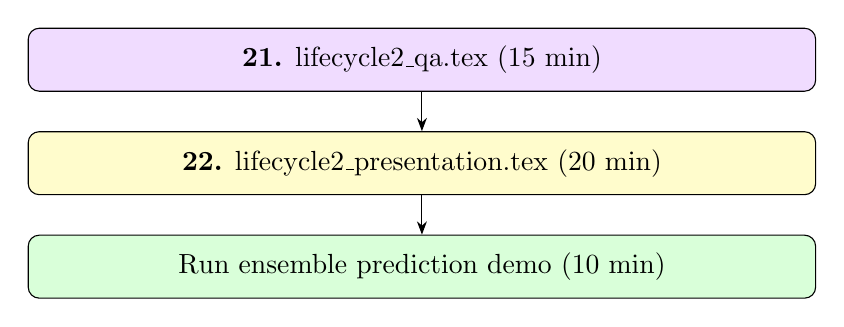
\begin{tikzpicture}[
    node distance=0.5cm,
    box/.style={rectangle, draw, rounded corners, minimum width=10cm, minimum height=0.8cm, align=center, fill=#1}
]
\node[box=phase5] (a) {\textbf{21.} lifecycle2\_qa.tex (15 min)};
\node[box=yellow!20, below=of a] (b) {\textbf{22.} lifecycle2\_presentation.tex (20 min)};
\node[box=green!15, below=of b] (c) {Run ensemble prediction demo (10 min)};
\draw[-{Stealth}] (a) -- (b);
\draw[-{Stealth}] (b) -- (c);
\end{tikzpicture}
\end{center}

\subsection*{Step 21: lifecycle2\_qa.tex $\bigstar$}
\begin{itemize}[leftmargin=1.5cm]
    \item[\textbf{Time:}] 15 minutes
    \item[\textbf{What you learn:}] LC2-specific questions: ``Why temperature scaling and not Platt scaling?'', ``Why 60-40 weights?'', ``Why ViT instead of another CNN?'' Ready answers.
\end{itemize}

\subsection*{Step 22: lifecycle2\_presentation.tex $\bigstar$}
\begin{itemize}[leftmargin=1.5cm]
    \item[\textbf{Time:}] 20 minutes
    \item[\textbf{Action:}] Compile PDF, click through all slides. Practice what to say on each. Includes: LC1 recap, temperature scaling, ensemble, ViT, confusion matrix + ROC plots, pipeline demo, cumulative table.
\end{itemize}

% ---- LC2 Presentation ----
\section{PRESENTATION DAY: Saturday, 29 March 2026 --- Lifecycle 2}

\noindent\fcolorbox{black}{lc2}{%
\parbox{\dimexpr\linewidth-2\fboxsep-2\fboxrule}{%
\textbf{What to show your guide:}
\begin{enumerate}
    \item Open \textbf{lifecycle2\_presentation.tex} PDF --- present all slides
    \item Start with: ``In LC1 we got 79.97\% with EfficientNet-B3. LC2 improves this to 84.55\%.''
    \item Show \textbf{temperature scaling} --- explain T=1.1511, what it fixes
    \item Show \textbf{ensemble formula} --- 60\% EfficientNet + 40\% ViT, threshold 46.7\%
    \item Show \textbf{confusion matrix + ROC curve} --- fewer missed landslides
    \item Show \textbf{cumulative table} r0 to r5 --- the progression story
    \item Run \textbf{live ensemble prediction} on terminal
    \item End with: ``Still 3 gaps remain --- class imbalance, single-pass fragility, black-box. LC3 fixes all three.''
\end{enumerate}
}}

\vspace{0.3cm}
\noindent\textbf{Key numbers to memorize:}
\begin{itemize}
    \item r3: T=1.1511, accuracy unchanged (calibration only)
    \item r4: 82.40\% acc, 72.97\% F1 (ensemble + threshold)
    \item r5: 84.55\% acc, 75.98\% F1, 91.50\% AUC (ViT ensemble) --- biggest single jump
\end{itemize}

% ============================================================
% ============================================================
\part*{LIFECYCLE 3 PREPARATION}
\addcontentsline{toc}{part}{Lifecycle 3 Preparation}
% ============================================================
% ============================================================

\noindent\fcolorbox{black}{lc3}{%
\parbox{\dimexpr\linewidth-2\fboxsep-2\fboxrule}{%
\centering\Large\textbf{LIFECYCLE 3 --- Present on Sunday, 7 April 2026}\\[0.1cm]
\normalsize Advanced Techniques \& Deployment Readiness (r6)\\
\textbf{Covers:} Focal Loss, TTA, Grad-CAM, multi-class experiment
}}

\vspace{0.3cm}
\noindent You have \textbf{9 days} (30 March -- 7 April). Spread across 4 study sessions.

% ---- LC3 Day 1 ----
\section{Days 30--31 March (Mon--Tue) --- Learn LC3 Techniques}

\begin{center}
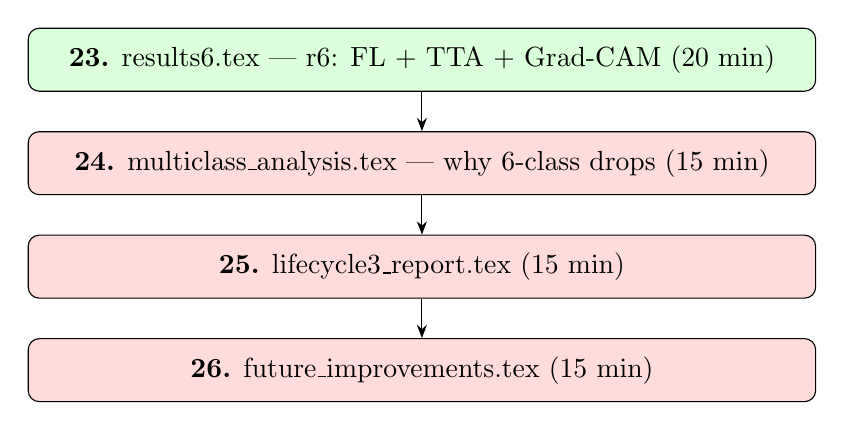
\begin{tikzpicture}[
    node distance=0.5cm,
    box/.style={rectangle, draw, rounded corners, minimum width=10cm, minimum height=0.8cm, align=center, fill=#1}
]
\node[box=phase3] (a) {\textbf{23.} results6.tex --- r6: FL + TTA + Grad-CAM (20 min)};
\node[box=phase4, below=of a] (b) {\textbf{24.} multiclass\_analysis.tex --- why 6-class drops (15 min)};
\node[box=phase4, below=of b] (c) {\textbf{25.} lifecycle3\_report.tex (15 min)};
\node[box=phase4, below=of c] (d) {\textbf{26.} future\_improvements.tex (15 min)};
\draw[-{Stealth}] (a) -- (b);
\draw[-{Stealth}] (b) -- (c);
\draw[-{Stealth}] (c) -- (d);
\end{tikzpicture}
\end{center}

\subsection*{Step 23: results6.tex (r6) $\bigstar$}
\begin{itemize}[leftmargin=1.5cm]
    \item[\textbf{Time:}] 20 minutes
    \item[\textbf{What you learn:}] Three techniques:
    \begin{itemize}
        \item \textbf{Focal Loss} ($\gamma=2.0$): down-weights easy examples, focuses on hard ones. Targets class imbalance.
        \item \textbf{TTA} (5 views): average predictions from original + flipped + rotated. Rescues borderline cases.
        \item \textbf{Grad-CAM}: heatmap showing where model looks. Red = high attention, Blue = low attention.
    \end{itemize}
    \item[\textbf{Also learn:}] Multi-class experiment (6 classes, dropped to $\sim$41\% --- see multiclass\_analysis.tex).
\end{itemize}

\subsection*{Step 24: multiclass\_analysis.tex $\bigstar$}
\begin{itemize}[leftmargin=1.5cm]
    \item[\textbf{Time:}] 15 minutes
    \item[\textbf{What you learn:}] Why binary gives 84.55\% but 6-class drops to 41\%. Three root causes: insufficient per-class samples ($\sim$120), visual similarity between subtypes, 13:1 class imbalance. What datasets exist. What approaches would fix it (hierarchical classification, NIR bands, more data). Includes a ready-made answer for your guide.
    \item[\textbf{Critical for Q\&A:}] If guide asks ``why is multi-class accuracy low?'' --- this file has the exact answer.
\end{itemize}

\subsection*{Step 25: lifecycle3\_report.tex $\bigstar$}
        \item \textbf{Grad-CAM}: heatmap showing where model looks. Red = high attention, Blue = low attention.
    \end{itemize}
    \item[\textbf{Also learn:}] Multi-class experiment (6 classes, dropped to 71.67\% --- insufficient per-class samples).
\end{itemize}

\subsection*{Step 24: lifecycle3\_report.tex $\bigstar$}
\begin{itemize}[leftmargin=1.5cm]
    \item[\textbf{Time:}] 15 minutes
    \item[\textbf{What you learn:}] LC3 as a coherent story. Train better + Predict better + Explain better.
\end{itemize}

\subsection*{Step 26: future\_improvements.tex}
\begin{itemize}[leftmargin=1.5cm]
    \item[\textbf{Time:}] 15 minutes
    \item[\textbf{What you learn:}] What could be done next --- NIR bands, larger datasets, pixel-level segmentation, real-time deployment. Good for ``what are your limitations?'' questions.
\end{itemize}

% ---- LC3 Day 2 ----
\section{Days 1--2 April (Wed--Thu) --- Deep Dives + Comparison}

\begin{center}
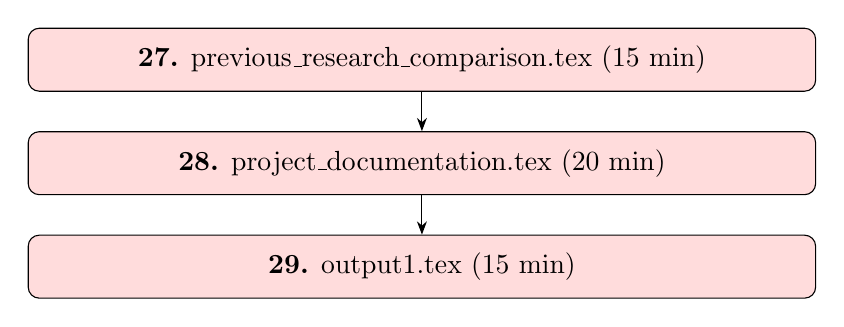
\begin{tikzpicture}[
    node distance=0.5cm,
    box/.style={rectangle, draw, rounded corners, minimum width=10cm, minimum height=0.8cm, align=center, fill=#1}
]
\node[box=phase4] (a) {\textbf{27.} previous\_research\_comparison.tex (15 min)};
\node[box=phase4, below=of a] (b) {\textbf{28.} project\_documentation.tex (20 min)};
\node[box=phase4, below=of b] (c) {\textbf{29.} output1.tex (15 min)};
\draw[-{Stealth}] (a) -- (b);
\draw[-{Stealth}] (b) -- (c);
\end{tikzpicture}
\end{center}

\subsection*{Step 27: previous\_research\_comparison.tex}
\begin{itemize}[leftmargin=1.5cm]
    \item[\textbf{Time:}] 15 minutes
    \item[\textbf{What you learn:}] How your project compares to published methods (NDVI, SVM, Random Forest, U-Net). Answers ``how is yours better?''
\end{itemize}

\subsection*{Step 28: project\_documentation.tex}
\begin{itemize}[leftmargin=1.5cm]
    \item[\textbf{Time:}] 20 minutes
    \item[\textbf{What you learn:}] Formal documentation --- problem statement, datasets, preprocessing. Good for final-lifecycle formality.
\end{itemize}

\subsection*{Step 29: output1.tex}
\begin{itemize}[leftmargin=1.5cm]
    \item[\textbf{Time:}] 15 minutes
    \item[\textbf{What you learn:}] Detailed single-image inference report --- TTA predictions, ensemble fusion, Grad-CAM explanation. Understand every number in the output.
\end{itemize}

% ---- LC3 Day 3 ----
\section{Days 3--5 April (Fri--Sun) --- Q\&A Prep + Presentation + Demo}

\begin{center}
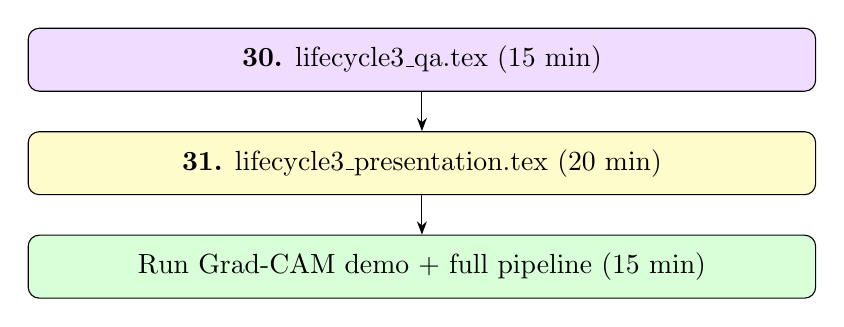
\begin{tikzpicture}[
    node distance=0.5cm,
    box/.style={rectangle, draw, rounded corners, minimum width=10cm, minimum height=0.8cm, align=center, fill=#1}
]
\node[box=phase5] (a) {\textbf{30.} lifecycle3\_qa.tex (15 min)};
\node[box=yellow!20, below=of a] (b) {\textbf{31.} lifecycle3\_presentation.tex (20 min)};
\node[box=green!15, below=of b] (c) {Run Grad-CAM demo + full pipeline (15 min)};
\draw[-{Stealth}] (a) -- (b);
\draw[-{Stealth}] (b) -- (c);
\end{tikzpicture}
\end{center}

\subsection*{Step 30: lifecycle3\_qa.tex $\bigstar$}
\begin{itemize}[leftmargin=1.5cm]
    \item[\textbf{Time:}] 15 minutes
    \item[\textbf{What you learn:}] LC3-specific questions: ``Why gamma=2 for Focal Loss?'', ``How many TTA views and why?'', ``What layer does Grad-CAM use?'', ``Why did multi-class fail?'' Ready answers. Also read multiclass\_analysis.tex for the detailed answer.
\end{itemize}

\subsection*{Step 31: lifecycle3\_presentation.tex $\bigstar$}
\begin{itemize}[leftmargin=1.5cm]
    \item[\textbf{Time:}] 20 minutes
    \item[\textbf{Action:}] Compile PDF, click through all slides. Includes: project journey, LC2 gaps, Focal Loss, TTA, Grad-CAM with heatmap image, full pipeline demo, evaluation plots, cumulative r0-r6 table, multi-class experiment, future improvements.
\end{itemize}

\subsection*{Live Demo Practice}
\begin{itemize}[leftmargin=1.5cm]
    \item[\textbf{Time:}] 15 minutes
    \item[\textbf{Action:}]
    \begin{enumerate}
        \item Run prediction: show Phase 1 + Phase 2 terminal output
        \item Open \textbf{gradcam\_ls\_test\_0011.png} --- explain: ``Red areas show where the model looks --- exposed soil and debris patterns. This matches the actual landslide.''
        \item Open confusion matrix + ROC curve
        \item Show the complete r0-to-r6 progression table
    \end{enumerate}
\end{itemize}

% ---- LC3 Presentation ----
\section{PRESENTATION DAY: Sunday, 7 April 2026 --- Lifecycle 3 (Final)}

\noindent\fcolorbox{black}{lc3}{%
\parbox{\dimexpr\linewidth-2\fboxsep-2\fboxrule}{%
\textbf{What to show your guide:}
\begin{enumerate}
    \item Open \textbf{lifecycle3\_presentation.tex} PDF --- present all slides
    \item Start with: ``LC1 built the foundation, LC2 optimized. LC3 makes it deployment-ready.''
    \item Show \textbf{Focal Loss} formula + example table (100x reduction for easy samples)
    \item Show \textbf{TTA} worked example (borderline 0.48 rescued to 0.51)
    \item Show \textbf{Grad-CAM side-by-side}: original image vs heatmap
    \item Show \textbf{full pipeline terminal output}: detection + type + forecast
    \item Show \textbf{complete r0--r6 table}: the full project story in one table
    \item Show \textbf{multi-class experiment}: honest about 71.67\% drop, explain why
    \item End with: future improvements (NIR bands, larger data, segmentation, real-time)
\end{enumerate}
}}

\vspace{0.3cm}
\noindent\textbf{Key numbers to memorize:}
\begin{itemize}
    \item Focal Loss: $\gamma=2.0$, reduces easy-sample loss by 100x
    \item TTA: 5 views (original, H-flip, V-flip, HV-flip, 90-degree rotation)
    \item Grad-CAM: EfficientNet-B3 gives 10x10 heatmap, ViT gives 14x14
    \item Multi-class: dropped from 84.55\% to 71.67\% (insufficient per-class samples)
    \item Total journey: 78.54\% (r0) to 84.55\% (r5), F1: 67.67\% to 75.98\%, AUC: 85.53\% to 91.50\%
\end{itemize}

% ============================================================
\part*{COMPLETE SCHEDULE AT A GLANCE}
\addcontentsline{toc}{part}{Complete Schedule}
% ============================================================

\begin{center}
\renewcommand{\arraystretch}{1.25}
\small
\begin{tabular}{llll}
    \toprule
    \textbf{Date} & \textbf{Day} & \textbf{Task} & \textbf{Time} \\
    \midrule
    \multicolumn{4}{c}{\cellcolor{lc1}\textbf{--- LIFECYCLE 1 ---}} \\
    19 Mar (Wed) & Day 1 & content, study\_guide, explanation, architecture & 1.5 hr \\
    20 Mar (Thu) & Day 2 & results (r0, r1, r2), LC1 report, Q\&A prep & 1.5 hr \\
    20 Mar (Fri night) & Day 3 & LC1 opening, presentation practice, live demo test & 1 hr \\
    \rowcolor{lc1} \textbf{21 Mar (Sat)} & \textbf{PRESENT} & \textbf{LIFECYCLE 1 to guide} & \\
    \midrule
    \multicolumn{4}{c}{\cellcolor{lc2}\textbf{--- LIFECYCLE 2 ---}} \\
    22--23 Mar (Mon--Tue) & Days 4--5 & results3, results4, results5 (r3, r4, r5) & 1 hr \\
    24--25 Mar (Wed--Thu) & Days 6--7 & LC2 report, comparison, metrics, threshold & 1 hr \\
    26--27 Mar (Fri--Sat) & Days 8--9 & LC2 Q\&A, presentation practice, demo & 1 hr \\
    28 Mar (Fri night) & Day 10 & Final revision + test demo & 0.5 hr \\
    \rowcolor{lc2} \textbf{29 Mar (Sat)} & \textbf{PRESENT} & \textbf{LIFECYCLE 2 to guide} & \\
    \midrule
    \multicolumn{4}{c}{\cellcolor{lc3}\textbf{--- LIFECYCLE 3 ---}} \\
    30--31 Mar (Mon--Tue) & Days 11--12 & results6 (r6), LC3 report, future improvements & 1 hr \\
    1--2 Apr (Wed--Thu) & Days 13--14 & research comparison, documentation, output1 & 1 hr \\
    3--5 Apr (Fri--Sun) & Days 15--17 & LC3 Q\&A, presentation practice, Grad-CAM demo & 1 hr \\
    6 Apr (Sat night) & Day 18 & Final revision + full demo test & 0.5 hr \\
    \rowcolor{lc3} \textbf{7 Apr (Sun)} & \textbf{PRESENT} & \textbf{LIFECYCLE 3 to guide (FINAL)} & \\
    \bottomrule
\end{tabular}
\end{center}

\vspace{0.5cm}
\noindent\fcolorbox{black}{green!10}{%
\parbox{\dimexpr\linewidth-2\fboxsep-2\fboxrule}{%
\textbf{Total study time:} $\sim$10 hours spread over 20 days\\
\textbf{Per lifecycle:} $\sim$3--4 hours of reading + 30 min demo practice\\
\textbf{Per day:} $\sim$1--1.5 hours (very manageable)
}}

% ============================================================
\section*{Complete File Reading Order (All 31 Files)}
% ============================================================

\begin{center}
\renewcommand{\arraystretch}{1.15}
\footnotesize
\begin{tabular}{cllcl}
    \toprule
    \textbf{\#} & \textbf{File} & \textbf{Topic} & $\bigstar$ & \textbf{For LC} \\
    \midrule
    1 & content.tex & Why this project & $\bigstar$ & LC1 \\
    2 & study\_guide.tex (Part 1--2) & ML basics + overview & $\bigstar$ & LC1 \\
    3 & explanation.tex & Pipeline explained simply & & LC1 \\
    4 & architecture\_explanation.tex & Technical architecture & $\bigstar$ & LC1 \\
    5 & results.tex & r0: AlexNet baseline & $\bigstar$ & LC1 \\
    6 & results1.tex & r1: AlexNet pretrained & & LC1 \\
    7 & results2.tex & r2: EfficientNet-B3 & $\bigstar$ & LC1 \\
    8 & lifecycle1\_report.tex & LC1 summary & $\bigstar$ & LC1 \\
    9 & guide\_qa\_preparation.tex & General Q\&A & $\bigstar$ & LC1 \\
    10 & lifecycle1\_qa.tex & LC1 Q\&A & $\bigstar$ & LC1 \\
    11 & lifecycle1\_opening.tex & Speaking guide & $\bigstar$ & LC1 \\
    12 & lifecycle1\_presentation.tex & LC1 slides & $\bigstar$ & LC1 \\
    13 & run\_guide.tex & How to run code & $\bigstar$ & LC1 \\
    \midrule
    14 & results3.tex & r3: Temperature scaling & $\bigstar$ & LC2 \\
    15 & results4.tex & r4: Ensemble + threshold & $\bigstar$ & LC2 \\
    16 & results5.tex & r5: ViT ensemble & $\bigstar$ & LC2 \\
    17 & lifecycle2\_report.tex & LC2 summary & $\bigstar$ & LC2 \\
    18 & comparison\_and\_metrics.tex & r0--r5 comparison & & LC2 \\
    19 & evaluation\_metrics.tex & Metrics deep dive & & LC2 \\
    20 & threshold\_analysis.tex & Threshold analysis & & LC2 \\
    21 & lifecycle2\_qa.tex & LC2 Q\&A & $\bigstar$ & LC2 \\
    22 & lifecycle2\_presentation.tex & LC2 slides & $\bigstar$ & LC2 \\
    \midrule
    23 & results6.tex & r6: FL + TTA + Grad-CAM & $\bigstar$ & LC3 \\
    24 & multiclass\_analysis.tex & Binary vs 6-class analysis & $\bigstar$ & LC3 \\
    25 & lifecycle3\_report.tex & LC3 summary & $\bigstar$ & LC3 \\
    26 & future\_improvements.tex & Future work & & LC3 \\
    27 & previous\_research\_comparison.tex & Literature comparison & & LC3 \\
    28 & project\_documentation.tex & Formal documentation & & LC3 \\
    29 & output1.tex & Inference report & & LC3 \\
    30 & lifecycle3\_qa.tex & LC3 Q\&A & $\bigstar$ & LC3 \\
    31 & lifecycle3\_presentation.tex & LC3 slides & $\bigstar$ & LC3 \\
    \bottomrule
\end{tabular}
\end{center}

\end{document}
